\PassOptionsToPackage{unicode=true}{hyperref} % options for packages loaded elsewhere
\PassOptionsToPackage{hyphens}{url}
\PassOptionsToPackage{dvipsnames,svgnames*,x11names*,table}{xcolor}
%
%\documentclass[a4paper,]{scrartcl}
\documentclass{article}

\usepackage{amssymb,amsmath}
\usepackage{ifxetex,ifluatex}
\usepackage{fixltx2e} % provides \textsubscript
\ifnum 0\ifxetex 1\fi\ifluatex 1\fi=0 % if pdftex
  \usepackage[T1]{fontenc}
  \usepackage[utf8]{inputenc}
  \usepackage{textcomp} % provides euro and other symbols
\else % if luatex or xelatex
  \usepackage{unicode-math}
  \defaultfontfeatures{Ligatures=TeX,Scale=MatchLowercase}
\fi
% use upquote if available, for straight quotes in verbatim environments
\IfFileExists{upquote.sty}{\usepackage{upquote}}{}

% use microtype if available
\IfFileExists{microtype.sty}{
\usepackage[]{microtype}
\UseMicrotypeSet[protrusion]{basicmath} % disable protrusion for tt fonts
}{}

\IfFileExists{parskip.sty}{%
\usepackage{parskip}
}{% else
\setlength{\parindent}{0pt}
\setlength{\parskip}{6pt plus 2pt minus 1pt}
}

\usepackage{xcolor}
\definecolor{default-citecolor}{HTML}{4077C0}
\definecolor{default-urlcolor}{HTML}{4077C0}

\usepackage{hyperref}
\hypersetup{
            pdftitle={The Raft Consensus Algorithm},
            pdfauthor={Fabio Anderegg},
            colorlinks=true,
            linkcolor=Maroon,
            citecolor=default-citecolor,
            urlcolor=cyan,
            breaklinks=true}
\urlstyle{same}  % don't use monospace font for urls
\usepackage[margin=2.5cm,includehead=true,includefoot=true,centering]{geometry}
\setlength{\emergencystretch}{3em}  % prevent overfull lines
\providecommand{\tightlist}{%
  \setlength{\itemsep}{0pt}\setlength{\parskip}{0pt}}
\setcounter{secnumdepth}{5}
% Redefines (sub)paragraphs to behave more like sections
\ifx\paragraph\undefined\else
\let\oldparagraph\paragraph
\renewcommand{\paragraph}[1]{\oldparagraph{#1}\mbox{}}
\fi
\ifx\subparagraph\undefined\else
\let\oldsubparagraph\subparagraph
\renewcommand{\subparagraph}[1]{\oldsubparagraph{#1}\mbox{}}
\fi

% Make use of float-package and set default placement for figures to H
\usepackage{float}
\floatplacement{figure}{H}


\title{The Raft Consensus Algorithm}
\author{Fabio Anderegg}
\date{2017-12-04}





%%
%% added
%%

%
% No language specified? take American English.
%

\ifnum 0\ifxetex 1\fi\ifluatex 1\fi=0 % if pdftex
  \usepackage[shorthands=off,main=english]{babel}
\else
  % See issue https://github.com/reutenauer/polyglossia/issues/127
  \renewcommand*\familydefault{\sfdefault}
  % load polyglossia as late as possible as it *could* call bidi if RTL lang (e.g. Hebrew or Arabic)
  \usepackage{polyglossia}
  \setmainlanguage[]{english}
\fi


%
% colors
%

%
% for the background color of the title page
%
\usepackage{pagecolor}
\usepackage{afterpage}

%
% TOC depth and 
% section numbering depth
%
\setcounter{tocdepth}{3}
\setcounter{secnumdepth}{3}

%
% line spacing
%
\usepackage{setspace}
\setstretch{1.2}

%
% break urls
%
\PassOptionsToPackage{hyphens}{url}

%
% When using babel or polyglossia with biblatex, loading csquotes is recommended 
% to ensure that quoted texts are typeset according to the rules of your main language.
%
\usepackage{csquotes}

%
% captions
%
\usepackage[font={small,it}]{caption}
\newcommand{\imglabel}[1]{\textbf{\textit{(#1)}}}

%
% blockquote
%
\definecolor{blockquote-border}{RGB}{221,221,221}
\definecolor{blockquote-text}{RGB}{119,119,119}
\usepackage{mdframed}
\newmdenv[rightline=false,bottomline=false,topline=false,linewidth=3pt,linecolor=blockquote-border,skipabove=\parskip]{customblockquote}
\renewenvironment{quote}{\begin{customblockquote}\list{}{\rightmargin=0em\leftmargin=0em}%
\item\relax\color{blockquote-text}\ignorespaces}{\unskip\unskip\endlist\end{customblockquote}}

%
% Source Sans Pro as the default font family
% Source Code Pro for monospace text
%
% 'default' option sets the default 
% font family to Source Sans Pro, not \sfdefault.
%
\usepackage[default]{sourcesanspro}
\usepackage{sourcecodepro}

%
% heading color
%
\definecolor{heading-color}{RGB}{40,40,40}
%\addtokomafont{section}{\color{heading-color}}
% When using the classes report, scrreprt, book, 
% scrbook or memoir, uncomment the following line.
%\addtokomafont{chapter}{\color{heading-color}}

%
% variables for title and author
%
\usepackage{titling}
\title{The Raft Consensus Algorithm}
\author{Fabio Anderegg}

%
% environment for boxes
%
%\usepackage{framed}

%
% tables
%

%
% remove paragraph indention
%
\setlength{\parindent}{0pt}
\setlength{\parskip}{6pt plus 2pt minus 1pt}
\setlength{\emergencystretch}{3em}  % prevent overfull lines

%
% header and footer
%
\usepackage{fancyhdr}
\pagestyle{fancy}
\fancyhead{}
\fancyfoot{}
\lhead{The Raft Consensus Algorithm}
\chead{}
\rhead{2017-12-04}
\lfoot{Fabio Anderegg}
\cfoot{}
\rfoot{\thepage}
\renewcommand{\headrulewidth}{0.4pt}
\renewcommand{\footrulewidth}{0.4pt}

\usepackage{graphicx}
\graphicspath{
{images/}
{scenarios/}
{scenarios/election/}
{scenarios/split_votes/}
}

\usepackage{enumitem}
\setitemize{noitemsep,topsep=0pt,parsep=0pt,partopsep=0pt}


\usepackage{tabularx}
\usepackage{calc}


\begin{document}

%%
%% begin titlepage
%%

\begin{titlepage}
\newgeometry{left=6cm}
\definecolor{titlepage-color}{HTML}{2196F3}
\newpagecolor{titlepage-color}\afterpage{\restorepagecolor}
\newcommand{\colorRule}[3][black]{\textcolor[HTML]{#1}{\rule{#2}{#3}}}
\begin{flushleft}
\noindent
\\[-1em]
\color[HTML]{FFFFFF}
\makebox[0pt][l]{\colorRule[1976D2]{1.3\textwidth}{8pt}}
\par
\noindent

{ \setstretch{1.4}
\vfill
\noindent {\huge \textbf{\textsf{The Raft Consensus Algorithm}}}
\vskip 2em
\noindent
{\Large \textsf{\MakeUppercase{Fabio Anderegg}}
\vfill
}

\textsf{2017-12-04}}
\end{flushleft}
\end{titlepage}
\restoregeometry

%%
%% end titlepage
%%


{
\hypersetup{linkcolor=}
\setcounter{tocdepth}{3}
\tableofcontents
\pagebreak
}

\section{Abstract}

Raft is a consensus algorithm for distributed systems. It aims to be easier to understand and implemented in real-world software than Paxos, an older and wildy used algorithm.

This paper explains the algorithm from the bottom up, first describing all the components and
then explaining how they work together to solve specific scenarios.

The paper describes the behaviour of the algorithm, especially the reaction to network messages
in great detail, including discussing edge cases. This should help programmers to implement
the algorithm because it requires much less cross-referencing information from multiple chapters in
comparison to the original paper and PhD thesis.

\section{Introduction}


\includegraphics[scale=0.05]{raft}

This paper covers Raft, a consensus algorithm for distributed systems.

Raft wants to be a simpler replacement for PAXOS, an algorithm developed by Leslie Lamport and considered the reference consensus algorithm for distributed systems\cite{paxos}. PAXOS suffers from two big problems, which Raft tries to solve: It is hard to understand \cite[p.91]{raft_phd_thesis}, has some missing pieces for a real world system and is generally hard to implement\cite{paxos_made_live}.

Raft was developed by Diego Ongaro and extensively described in this PhD thesis \cite{raft_phd_thesis}. He not only describes how the algorithm works, but also did a study under students to test if the algorithm is actually easier to understand than PAXOS. Raft has been formally verified \cite{raft_proof} and implemented in multiple real world systems, e.g. in etcd \cite{etcd_raft}, Consul \cite{consul_raft} and RethinkDB \cite{rethinkdb_raft}.

The offical GitHub Page \cite{raft_github} contains many further references about the algorithm, a simulator for the algorithm from which screenshots have been used in this paper and an extensive list of implementations in many different programming languages.

This paper has three main parts: The first part explains what consensus in a distributed system means, the second part explains how the Raft algorithm works in detail and the third part shows how the algorithm reacts to some specific scenarios.
The pictures for the scenarios sections were created using Raftscope \cite{raftscope}, a software to visualize the state of Raft-based distributed system.

This paper describes the latest version of Raft as described in Diego Ongaros PhD dissertation \cite{raft_phd_thesis}. Compared to the papers published before the dissertation, the dissertation describes the client-cluster interaction much more clearly and contains a simpler cluster membership change algorithm.

\subsection{What is consensus?}

Consensus in a distributed system means that multiple servers agree on the same specific state of the system. After agreeing on a state, that state cannot be changed any more, but the system can agree on a new state superseding the old state.

Clients interacting with such a system see a single consistent state, independent of the server they are talking to.

This problem is hard to solve because most components participating in the system (servers, network, clocks, disk...) are inherently unreliable. They can not only fail and be complete unusable, they can also be slow, mangle data in transit (network packets ordering) or contain invalid data (bit flipping in RAM).

Many consensus algorithms (including Raft) are based on a majority system. If a majority of the servers agree on a specific value, that value is considered the "true" value of the system.

\subsection{The CAP Theorem}
The CAP theorem describe how certain failures in a distributed system affect the system. It states that a distributed system can never provide more than two of the following guarantees: \cite{cap_theorem}

\textbf{Consistency}: Operations in the system must appear as if they happened one after another in total order. At a specific time all servers must return the same, most recent write to the system.

\textbf{Availability}: Every working node in the system must be able to return a response to a request.

\textbf{Partition tolerance}: The system works even when the network drops packets, loses nodes or is partitioned.

Raft is a CP algorithm, that means systems using this algorithm are tolerant to partitions and always return a consistent view of the data in the system. Raft sacrifices the availability guarantee, which means that at least a majority of the servers must be working and be able to communicate with each other for the system to be usable.

\section{The algorithm}
A Raft cluster consists of nodes. A node is a server running the Raft software and communicating with the other nodes in the cluster over a network connection.
Every one has a unique ID which is used in the election process. In every cluster, one node is elected as a leader node, which coordinates the operations inside the cluster. A leader can only be elected by
a majority of the cluster nodes. This means the minimal cluster size is three nodes, and bigger clusters should always have an uneven count of nodes (In a cluster
of six nodes, two nodes can crash and a majority can still be found, this is not better than a five node cluster, where also two nodes can crash without impacting the cluster).
This also means that when more than half of the cluster nodes are offline, the cluster is inoperable.
This is availability guarantee of the CAP theorem the Raft algorithm gives up for the other two guarantees.

Every leader is elected for a specific term. A term is a positive integer, incremented every time a node starts an election process by proposing itself as a new leader to the other nodes.

The current leader sends out a heartbeat network packet in some preconfigured interval. If a follower node does not receive a heartbeat within a given interval (which should be a bit longer than the interval in which the master sends out the heartbeats to account for the network round-trip time), the node considers the master to be down and proposes itself as a new leader.

The main data structure of the algorithm as a replicated, append-only log. It contains the data the clients wants to save in the system and also some metadata
for the algorithm itself.

The Raft algorithm is designed to survive the following and many other failure cases:
\begin{itemize}
    \item The current leader crashes
    \item Network connections between nodes fails
    \item Network connections are very slow or drop messages between nodes
\end{itemize}

\subsection{State}
Every node in the Raft cluster is always in one of the following three states:
\begin{itemize}
    \item Leader: The node is the leader of the cluster
    \item Candidate: The node did not receive a heartbeat from a leader, it is waiting to get enough votes to be a leader itself
    \item Follower: Some other node is a leader
\end{itemize}

\subsubsection*{Persistent data written to disk}

This data has to be saved on disk before replying to the RPC call from the leader. The fsync or equivalent system call should be used on the file descriptor to make sure the data has arrived on the disk and not just the write caches of the operating system [CN].

\begin{tabular}{ | l | p{13.7cm} | }
\hline
currentTerm & The election term the node thinks is the current one \\ \hline
votedFor & For which node the current node has voted in this term \\ \hline
log[] & The replicated log containing all the data clients want to save in the system. The log is append only, only new entries can be append but old ones can not be changed.
Every log entry contains an index (starting at one) and the term in which the data was written. \\ \hline
\end{tabular}

\subsubsection*{Volatile data}

This data is not written to disk and initialized on node startup.

\begin{tabularx}{\textwidth}{  | p{80px} | X | }
\hline
commitIndex & Up to which index in the replicated log the current node considers to be committed (commited means a majority of the cluster
received the data entry, saved it to disk and notified the leader). On startup, this information is initialized from the leaders heartbeat message (AppendEntry). \\
\hline
lastApplied & The highest index in the replicated log, initialized when reading the log entries from disk on startup. \\
\hline
receivedVotes[] & Vote responses per node id, a vote could be granted or rejected \\
\hline
\end{tabularx}

\subsubsection*{Leader data}

This data is initialized when the node gets elected as leader and is not persisted to disk.
It has to be cleared every time the node gets elected and must not be reused in later terms.

\begin{tabular}{ | l | p{13.7cm} | }
\hline
nextIndex[] & Index of the next entry the leader will send to the specific follower. This map/associative array is initialized to the leaders last log entry index + 1 on leader election.
This map is used when a followers log falls behind the leaders log and the leader starts to send missing log entries to the follower. \\ \hline
matchIndex[] & Index of the latest acknowledged (written to disk) log entry for the specific follower. Initialized to zero on leader election. \\ \hline
\end{tabular}

\subsection{Timers}
The Raft server needs two timers which when they run out trigger some action.

\subsubsection*{Election timer}
After a leader has been elected, it will send out heartbeat messages to all followers. This heartbeat
will restart the election timer running on the followers. If the timer runs out because the follower did not 
receive a heartbeat, the node will switch into candidate state and begin the election process to become a leader itself.
The election timer is inactive when the node is a leader.

The actual timeout in milliseconds has to be defined randomly. The minimum should be the network round-trip time between two nodes plus some margin,
and on top of that a random offset. The timeout should not be too high, because it influences the time the system requires to reelect a new leader
if the old one crashes. The minimal timeout and the random range should be configurable, because it highly depends on the environment where the algorithm runs
(network latency, server latency/performance etc.).

The actual timeout amount has to be random to avoid split votes where multiple nodes switch into candidate mode at the same time and the votes get split
up between these nodes. If this happens it is possible that no node receives the majority of the votes and the election process has to be restarted,
making the time where the cluster has no leader longer. This can still happen with randomized timeouts, but the chances are much smaller.

\subsubsection*{Candidate and leader timer}
This timer replaces the election timer when the node is a leader. In candidate state, both timers are active.
The timeout amount has to be smaller than the minimal election timeout. Half of the minimal election timeout is a good start.

In candidate mode, this timer is used to resend a RequestVote request message (see next chapter) if a node did not respond to the previous one.

In leader mode, this timer is used to periodically send out heartbeat messages to all followers.

\subsection{Network communication}

The communication between cluster nodes uses a remote procedure call (RPC) systems with two request and two corresponding response messages/packets. A RPC system with request/responses is required because handling of some responses require knowledge of the data sent in the request.

Clients interacting with the cluster add additional RPC calls and some optional extensions (like cluster membership) can also add additional calls.

The first message pair is RequestVote which is used in the voting process. The request is sent out ony by nodes in candidate state.
The second pair is AppendEntries which is sent out by the master as a heartbeat message and also to append data to the distrbuted log[] data structure.

\subsubsection*{RequestVote RPC call}
The RequestVote RPC call is used in the election process. When the election timer of a node expires, the node will do the following things:

\begin{itemize}
    \item Switch to candidate state
    \item Increment its currentTerm property by one
    \item Sets votedFor property to its own node id
    \item Reset the election timer
    \item Send out RequestVote requests to all other nodes
\end{itemize}

\textbf{Request}

\begin{tabular}{ | l | p{13.7cm} | }
\hline
term & Current term of the candidate \\ \hline
candidateId & Node id of the candidate \\ \hline
lastLogIndex & Index of the last applied log entry (could be uncommitted) \\ \hline
lastLogTerm & Term of the last applied log entry (could be uncommitted) \\ \hline
\end{tabular}

\textbf{Response}

\begin{tabular}{ | l | p{13.7cm} | }
\hline
term & The current term the answering node is in \\ \hline
voteGranted & If the answering node votes for the requesting node \\ \hline
\end{tabular}

\textbf{Request handling}

The first thing a node receiving a RequestVote request does is comparing its own term with the term in the request. If the term in the request is smaller than its own, it will reject to vote for this node by sending back a response with its current term and voteGranted flag set to false. The lower term value in the request is an indicator that the node sending the request is not up to date with the cluster and should therefore not be elected as a leader.

If the receiving node is a candidate or leader and the term in the request is higher than its own term, it will immediately switch to follower state and stop sending out heartbeat requests.
As above, a higher term value is an indicator for the \textit{receiving} node that it is behind the other nodes in the cluster and should not be a leader in this cluster.

If the currentTerm is the same as the term in the request and the votedFor property is already set to some node id, the request will also be rejected by responding with voteGranted set to false.

The last check is if the lastLogIndex and lastLogTerm are the same or higher than the latest entry in the nodes log[]. If yes, the node response with voteGranted set to true. This check is used to make sure a node is only elected as leader when it has the most recent data in the log.

If the node responds with a successful vote (voteGranted is true), it will also reset its own election timer.

\textbf{Candidate response handling}

If the term received in the response is higher than its own term, the node will switch to follower mode and therefore gives up to become a leader in the current term.

If the node does not receive enough votes (because more than half of the nodes are not accessible or the other nodes have a higher term), the election timer will run out again and a new election cycle is started.

The candidate tracks its received vote answers in the receivedVotes[] associative array/map. This array
saves if a node in the cluster voted for or against election the candidate as a new leader. If
the candidate receives enough notes, it switches to leader state and starts to send out hearbeat messages. This array is also used to resend RequestVote requests to nodes which did not respond in time,
which is measured using the candidate timer described above.

\subsubsection*{AppendEntries RPC call}
The AppendEntries RPC call is used by the master as a heartbeat message and also for
inserting data into the cluster log. It receives new data from a client and sends it out
to all followers. If enough followers acknowledge that they received the data, the leader
considers the data as committed and will signal to all followers in the next AppendEntry request 
that they should also consider the data committed.

\textbf{Request}

\begin{tabular}{ | l | p{12.7cm} | }
\hline
term & The leaders currentTerm \\ \hline
leaderId & The node id of the leader \\ \hline
prevLogIndex & Index of the log entry directly before the new ones in entries[] \\ \hline
prevLogTerm & Election term of the log entry directly before the new ones in entries[] \\ \hline
entires[] & The new data to be appended to the log, blank in heartbeat messages \\ \hline
leaderCommit & The commitIndex of the leader \\ \hline
\end{tabular}

\textbf{Response}

\begin{tabular}{ | l | p{13.7cm} | }
\hline
term & The responding nodes currentTerm \\ \hline
success & If the request succeeded \\ \hline
\end{tabular}

\textbf{Request sending}

The leader sends out AppendEntries when the heartbeat timer runs out or when a client sends new data. In both cases the request to the followers is constructed in the same way. When the request is sent out because the leader received new data from a client, it first appends the new data to its own log[]. Next, it starts to build the request to all followers: The prevLogIndex field is set to the value in nextIndex[] array for the specific node minus one, prevLogTerm is set to the corresponding term of the log entry. The entries[] field is now filled up with data from the leaders[] log starting with the index in nextIndex[] for the node.

\textbf{Request handling and response sending}

As in the VoteRequest request handling, the first action is to check if the term of the
leader in the request is smaller than currentTerm of the current node. If yes, a response with success
set to false is sent back.

Next, the follower checks if it has an entry in his log with index prevLogIndex and this entry having the term prevLogTerm.
If there is an entry but the term is incorrect, the follower removes this entry and all following entries and responses
with success set to false. If the follower has no entry with this index/term, it will also answer with success set to false.
The leader will start to send the missing log entries (see "Log data catch up" section below).

If the follower has the entries referenced in prevLogIndex and prevLogTerm, it will append the data in the entries[] field to his
own log. These entries are not committed yet, because it is possible that only a minority of the nodes in the cluster has the new data.

If the leader receives enough successful AppendEntry responses, it will increase its own commitIndex and send that out in the next AppendEntry request (heartbeat or with new data) in the leaderCommit field. When the checks above (term and prevLogIndex/prevLogTerm) are successful, the follower will set its own commitIndex to the one in leaderCommit.

\textbf{Response handling}

If the term in the response is higher than the currentTerm of the leader, the leader steps down immediately. The higher term
is an indicator that the leader is not up to date with the rest of the cluster.

If the success field is set to true, the leader records the highest written index (prevLogIndex + count of sent entries in the request) in its matchIndex[] array and
the same value plus one in the nextIndex[] array.

If enough nodes (the majority of the cluster including the leader) acknowledge the new data (can be checked using the matchIndex[] array), the leader will increase its commitIndex which will then be sent out to all nodes on the next AppendEntries request.

\textbf{Log data catch up}

If success in the response of the AppendEntry request is false, the data of the follower is not up to date or contains invalid data. The leader will begin sending out AppendEntries requests with lowered prevLogIndex/prevLogTerm every time until the follower finds a log[] entry matching with them. After that, the leader will start sending out log entries until the follower has the exact same log as the leader. This process uses the nextIndex[] array on the leader.





\section{Cluster membership}
Until now, the described algorithm uses a predefined cluster configuration with a given number of nodes. In a real-world system, it is desirable to
be able to add and remove nodes from the cluster. A use-case for this is e.g. replacing nodes for software updates or hardware upgrades or to
scale a cluster over more nodes for better performance.

The PhD dissertation \cite{raft_phd_thesis} describes in detail how such cluster membership changes can be implemented.
The algorithm is quite complex because it has to avoid certain failure cases when adding/removing cluster members:

\begin{itemize}
    \item Only adding one server at a time should be allowed to avoid two groups of nodes to be formed which would allow two leaders in the systems to be elected
    \item Removing a leader should be possible without interrupting the cluster operation
    \item Added servers should not be allowed to be elected as leaders because they have not yet catched up on the data
\end{itemize}

The algorithm for cluster membership is not as fleshed out as the core algorithm and contains many recommendations and ideas how things could be done, and not 
concrete explanations how something should be implemented. This requires some design decisions and experimentation from the programmer when creating a real-world implementation.


\section{Client interaction}

Until now, we only describe how nodes inside the cluster communicate with each other. To make the cluster actually usable from outside the cluster, some challenges have to be solved which are described in this chapter.

\subsection{Cluster discovery}
The first challenge for the client is to find the cluster. When the cluster is static and does not support member changes (see next chapter), this can be done by simply hard-coding the IP addresses of the cluster members in the client configuration. Resolving IP addresses using the domain name system would also be a possibility. This approach can also be used with changing cluster memberships, by updating the DNS records on changes.

\subsection{Leader discovery}
Only the leader in a Raft cluster can actually add new data to the log[]. One solution for this problem is that every node which gets contacted by a client but is not a leader acts as a proxy for the client and routes the requests to the master. Another solution is responding with the node id of the current leader. The node id of the leader is sent to all followers in the AppendEntry heartbeat message and can be sent out to clients.

\subsection{Writing data}
After finding the leader, a client sends data to leader. The leader adds the data to the Raft log and replicates the data to the cluster by sending out AppendEntries messages. Only when the leader receives an successful answer from a majority of the nodes in the cluster, it returns a success response message to the client.

\subsection{Duplicate writes}
Another guarantee the Raft algorithm tries to make is linearizability, which means a write of new data is executed exactly once. To implement this, a client registers with the cluster when first connecting. The cluster then creates a client session in memory. When the client sends a request to write some data, the request contains a unique request id. This request id is saved in the session. The session will be checked every time a new request from this client comes in to avoid duplicate writes from the same client by checking if the request id is already in the session.

A duplicate write can happen when a majority of the followers acknowledge the write, but the leader never sends back a success response message, because the leader crashed or the network between the client and the leader stopped to work.

For real-world implementations, it is important to remove sessions from clients which are not active any more, to avoid running out of memory. There are different approaches how to implement this, some are described in the PhD thesis\cite{raft_phd_thesis}, chapter 6.3.

\subsection{Inconsistens/stale reads}
(adressed in paper)
https://github.com/coreos/etcd/issues/741
https://aphyr.com/posts/316-call-me-maybe-etcd-and-consul
https://gist.github.com/armon/11059431

\section{Scenarios}
This section takes a look on different scenarios and failure modes in the cluster and how Raft handles these cases.

The small circles are the cluster nodes. The number inside the circle is the current term the node is in, the number outside the circle is the node id. The line around the circles show the election timer.

\newcommand{\raftscope}[2]{
  \begin{tabularx}{\textwidth}{  p{120px}  X  }
    \noindent\parbox[c]{\hsize}{
      \def\svgwidth{120}
      \fontsize{9pt}{11pt}\selectfont
      \input{#1}
    } & #2
\end{tabularx}
}

\subsection{Startup and leader election}


\raftscope{scenarios/election/40.pdf_tex}{
On cluster start up, there is no leader and all nodes are in the follower state.
}

\raftscope{scenarios/election/60.pdf_tex}{
After some time, one (or more, see split vote section below) nodes (S1) election timer will run out.
The node will switch to candidate mode and send out RequestVote request messages (green points)
}

\raftscope{scenarios/election/65.pdf_tex}{
All followers vote for this candidate by sending back a successful RequestVote response.
}

\raftscope{scenarios/election/72.pdf_tex}{
The node S1 is now elected as leader and starts to send out AppendEntries heartbeat messages.
}


\subsection{Leader crash}
A leader crash is handled exactly like the initial leader election.
After the leader crash, one of the follower nodes election timer will run out, because the node did not receive a heartbeat (AppendEntry) message from a leader. The node then sends out 
RequestVote packets and gets elected as the new leader.

\subsection{Split vote}

\raftscope{scenarios/split_votes/53.pdf_tex}{
TODO
}

\raftscope{scenarios/split_votes/68.pdf_tex}{
TODO
}

\raftscope{scenarios/split_votes/116.pdf_tex}{
TODO
}

\raftscope{scenarios/split_votes/126.pdf_tex}{
TODO
}

\raftscope{scenarios/split_votes/135.pdf_tex}{
TODO
}

\raftscope{scenarios/split_votes/139.pdf_tex}{
TODO
}

\subsection{Data write}
Writing data into the cluster uses the same message as the heartbeat.
* send out data
* reply with success
* update commit index in next appendentry heartbeat
* nodes update commit index

\subsection{Network partition}



\begin{tabularx}{\textwidth}{ |X|X| }
  \hline
  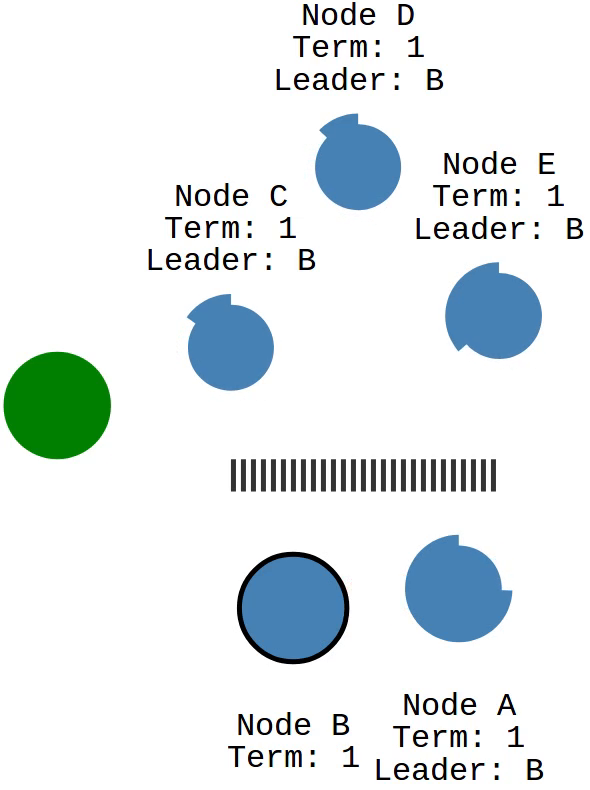
\includegraphics[scale=0.3]{scenarios/network_partition/0380.png} &
  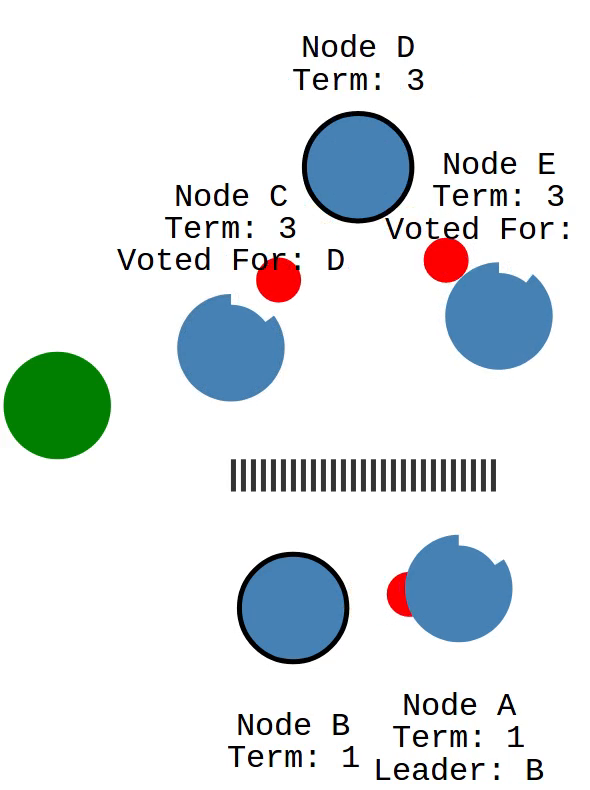
\includegraphics[scale=0.3]{scenarios/network_partition/0749.png} \\
  1. Initially, the cluster has one elected master and 5 working nodes. A network partition is introduced between the mast  &
  2. TODO 2  \\
  \hline
  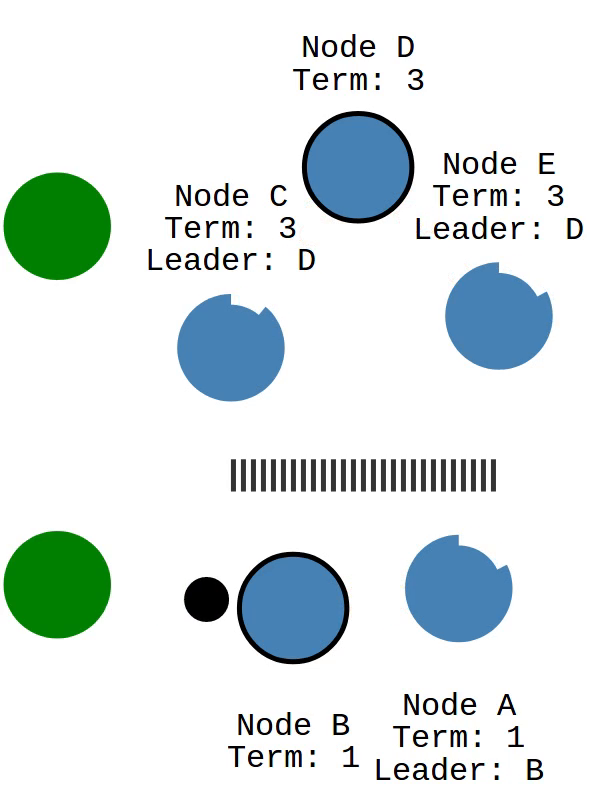
\includegraphics[scale=0.3]{scenarios/network_partition/1183.png} &
  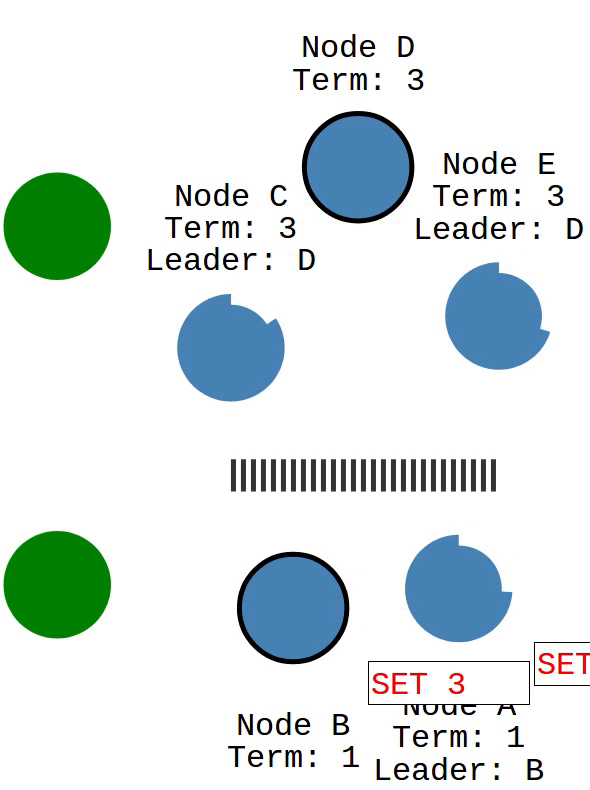
\includegraphics[scale=0.3]{scenarios/network_partition/1656.png} \\
  3) TODO 1  &
  4) TODO 2  \\
  \hline
\end{tabularx}

\begin{tabularx}{\textwidth}{ |X|X| }
  \hline
  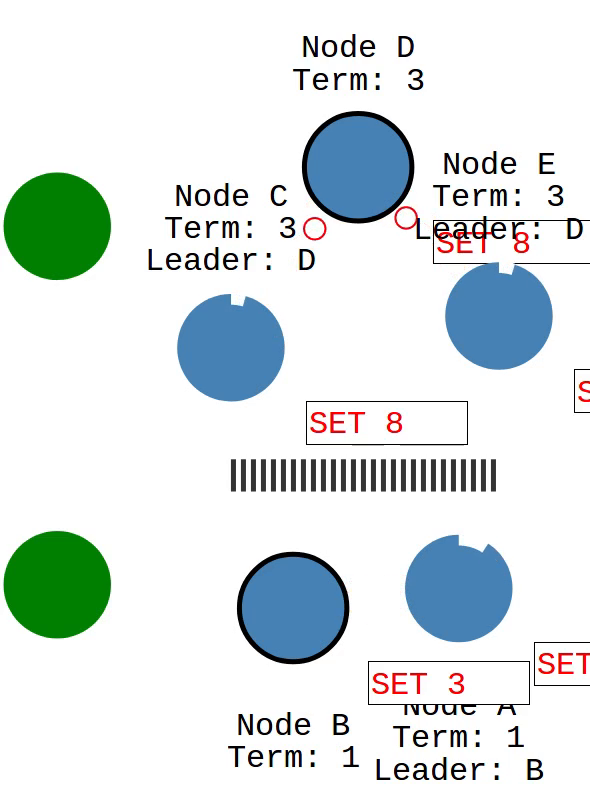
\includegraphics[scale=0.3]{scenarios/network_partition/1830.png} &
  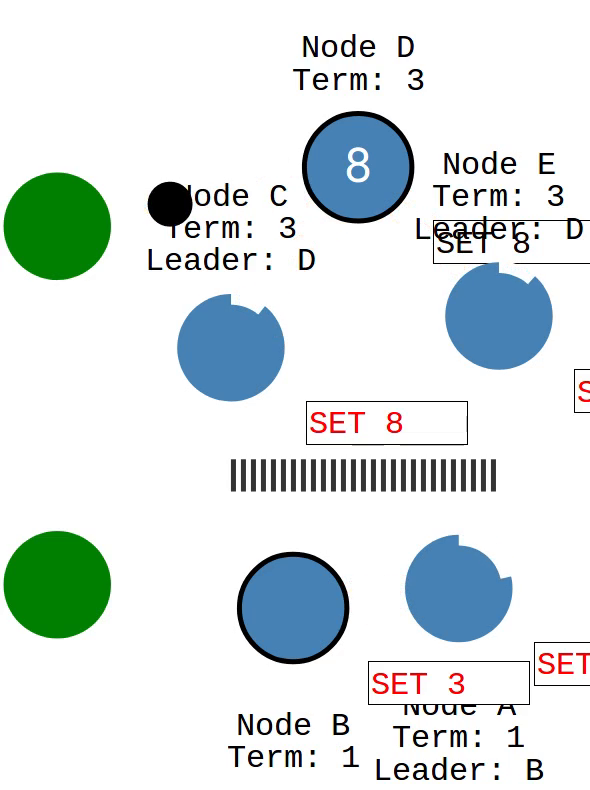
\includegraphics[scale=0.3]{scenarios/network_partition/1859.png} \\
  5) TODO 1  &
  6) TODO 2  \\
  \hline
  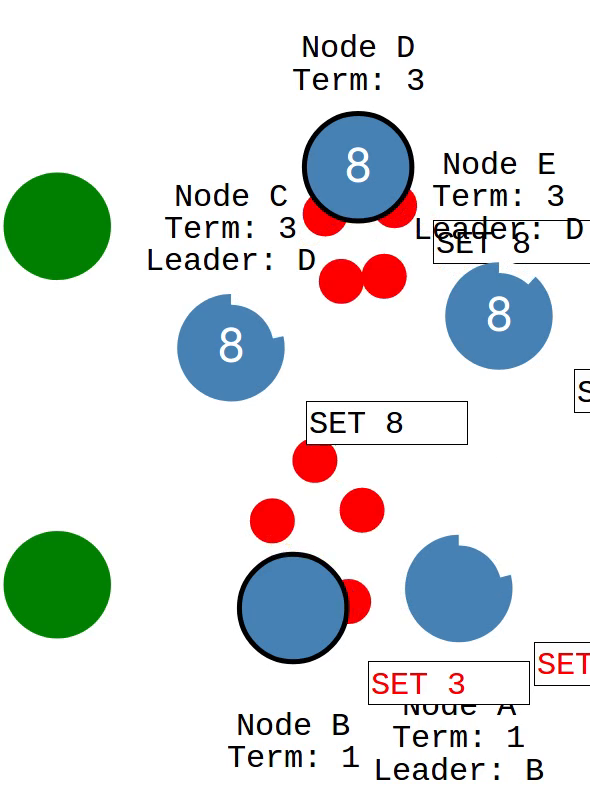
\includegraphics[scale=0.3]{scenarios/network_partition/2163.png} &
  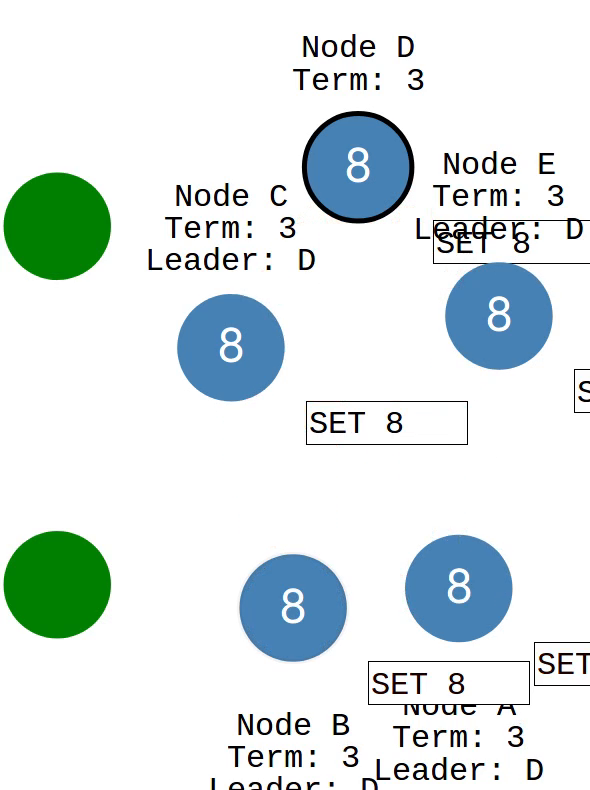
\includegraphics[scale=0.3]{scenarios/network_partition/2200.png} \\
  TODO 1  &
  TODO 2  \\
  \hline
\end{tabularx}


\section{Implementation}

Two attempts: C++ and Python
Difficulties:
Retrying requests/connects
Network timeout
Timer and request handling at the same time
Async programming or threads
State locking
Extremely difficult to test

\section{Conclusion}
Today, there are multiple real-world implementations of distributed systems using the Raft algorithm, proving that one of the main goals of Raft have been accomplished.

Kubernetes, a container management system initially developed by Google and now having a broad support in the IT community uses etcd, a key-value store written in Go and implementing the Raft algorithm, as its only database. Consul, a similar service to etcd can be used as a replacement in Kubernetes. Consul also uses the Raft algorithm.
Both systems are CP systems as described in the Raft paper.

Many newer databases from the NoSQL movement are also using the Raft algorithm, including MongoDB \cite{mongodb_raft}, CockroachDB\cite{cockroachdb_raft} and RethinkDB\cite{rethinkdb_raft}. For performance reasons, some of these databases use Raft for coordination inside the cluster, but not for the actual data replication\cite[Development section]{rethinkdb_raft_metadata}.

Diego Ongaro did a user study for his PhD thesis to prove that the algorithm is easier to understand than Paxos \cite[Raft user study chapter]{raft_phd_thesis}. The author of this paper also thinks that the algorithm is understandable, but by no means simple. Besides the original paper and the PhD thesis, the visualization Raftscope \cite{raftscope} and The Secret Lives of Data \cite{the_secret_lives_of_data} helper quite a bit, as did the source code of LogCabin\cite{logcabin}, the Raft implementation Ongaro wrote for his thesis.

\bibliographystyle{plain}
\bibliography{bibliography} 

\end{document}
